\documentclass[10pt, a4paper]{aqademic}

\usepackage[spanish]{babel}
	\selectlanguage{spanish}

% Document packages

\usepackage{amsmath}
\usepackage{amsfonts}
\usepackage[type=CC, modifier=by-nc-sa, version=4.0]{doclicense}
\usepackage{graphicx}
	\graphicspath{{img/}}

% Document settings

\author{Romero Lara, Rubio Gil}
\title{Desarrollo de Software}

\AqSetChapter{Práctica}

% Document composition

\begin{document}

\AqMaketitle[%
	author   = Clara María Romero Lara{,} Atanasio José Rubio Gil,
	cover    = logo-ugr.png,
	org      = Grado en Ingeniería Informática,
	subtitle = Prácticas,
	url      = https://github.com/Groctel/DS21
]
\tableofcontents

\chapter{Patrones de diseño}
\section{Filtro}

\section{Método factoría}

\begin{figure}[ht!]
\begin{center}
	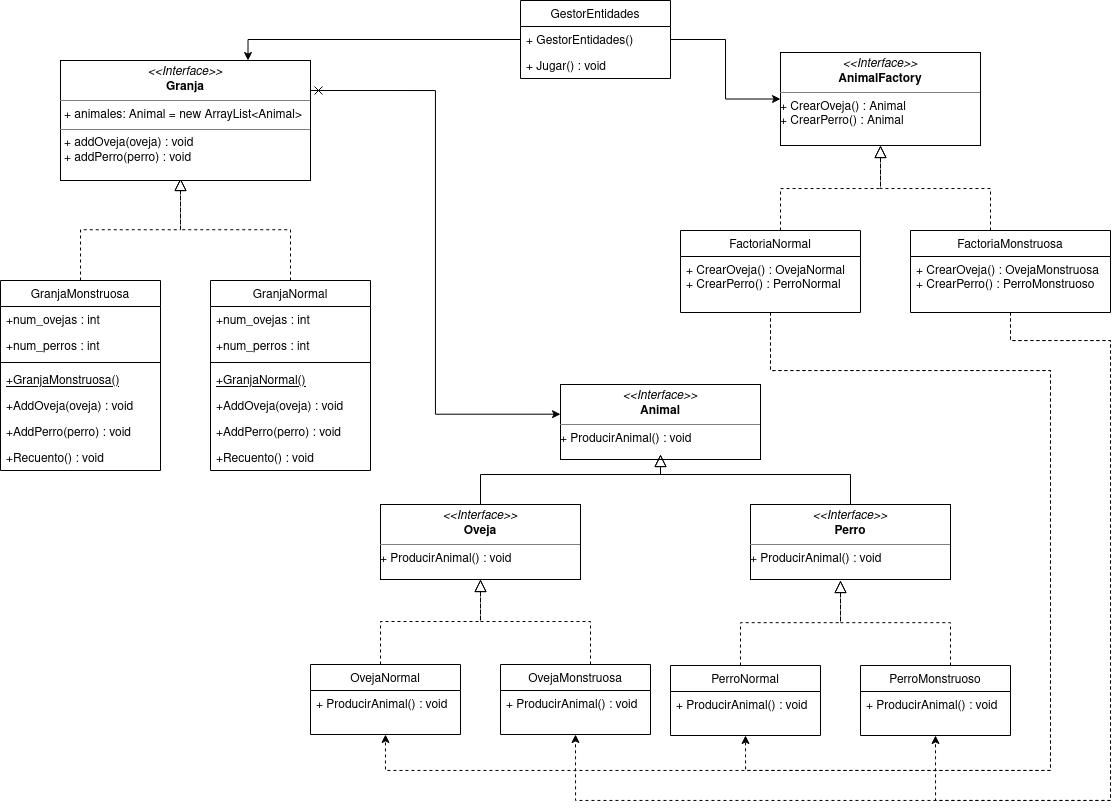
\includegraphics[scale=0.35]{DiagramaFactoria}
\end{center}
\caption{Diagrama UML de la aplicación del patrón \textit{Método Factoría}.}
\end{figure}

Hemos aplicado el patrón de diseño \textit{Método Factoría} sobre el sistema de gestión de entidades de \textit{CaveArt}, particularmente para la creación de granjas de animales.

Este procedimiento sería también aplicable a la generación de otras entidades pacíficas y hostiles, pero nos hemos decantado por este caso particular dado el valor añadido del concepto de la Granja. Además, estos otros casos serían más \textit{straightforward} y, por tanto, triviales.

El programa consiste en dos hebras concurrentes que llenan dos granjas: una \texttt{GranjaNormal}, habitada por ovejas y perros normales; y una \texttt{GranjaMonstruosa}, habitada por ovejas y perros monstruosos, hostiles al jugador.

Cada hebra del \texttt{GestorEntidades} llama a una factoría: \texttt{FactoriaNormal} o \texttt{FactoriaMonstruosa}. Estas factorías son implementaciones de la interfaz \texttt{AnimalFactory}. Se escoge de forma aleatoria si se generará una oveja o un perro, y la factoría llama al método \texttt{crearOveja} o \texttt{crearPerro} . Estos métodos, a su vez, llamarán al constructor del animal escogido.

\section{Observador}

\section{Prototipo}

\begin{figure}[ht!]
\begin{center}
	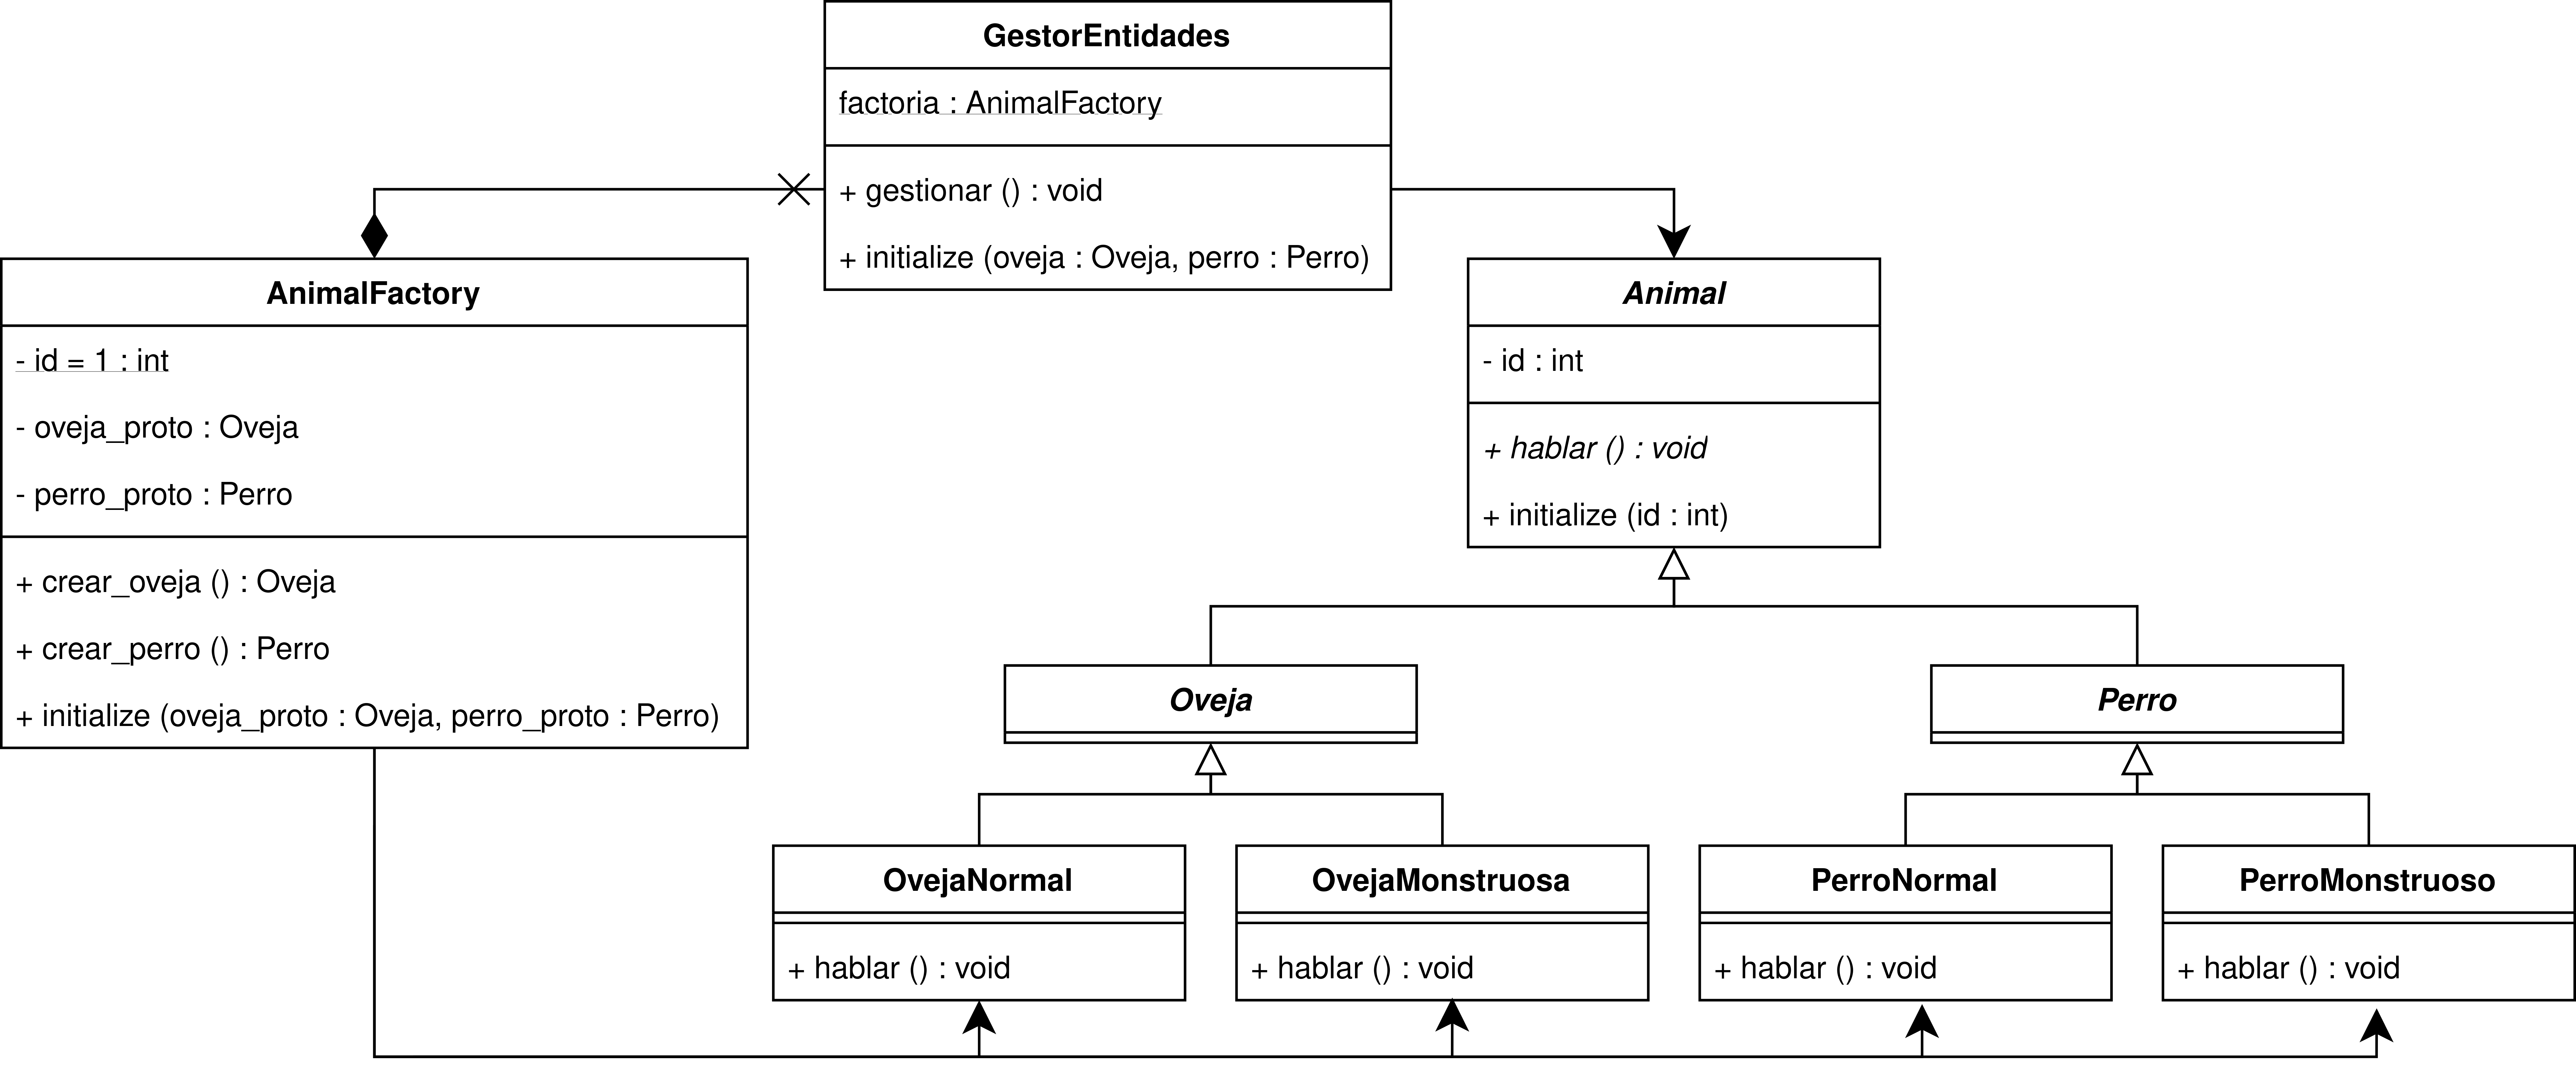
\includegraphics[scale=0.05]{DiagramaPrototipo}
\end{center}
\caption{Diagrama UML de la aplicación del patrón \textit{Prototipo}.}
\end{figure}

Nuestra aplicación del patrón \textit{Prototipo} consiste en una demo del sistema de creación de animales de \textit{CaveArt}.
Al inciar el programa, le preguntamos al jugador qué tipo de animales quiere y los almacenamos en \texttt{AnimalFactory} como prototipos.
Cuando esta clase crea los animales, llama al método \texttt{::clone} que tienen las clases por defecto en Ruby\footnote{%
	No hemos incluido \texttt{::clone} en el diagrama UML por no ser un método definido por nosotros.
}.

En la demostración puede verse fácilmente cómo cada animal se comporta de forma distinta en función de su naturaleza, imprimiendo un texto distinto en su método \texttt{::hablar}.


\end{document}
